\section{The cached finite field}
\label{sec:cached}

\subsection{Representation and tables}

The original element stores a polynomial. The cached element stores a 16-bit index, the
position of the element in the numbering the library already defines for
\code{from\_index}: for coefficients $c_0, c_1, c_2$ the index is $c_0 + 11c_1 + 121c_2$.
Zero is index 0.

Each operation has a table. Addition and multiplication have one slot per ordered pair of
operands, $q^2$ slots each for a field of $q$ elements. Negation and reciprocal have $q$
slots each. A slot holds 0 until its result is known and the index of the result plus one
afterwards. Listing~\ref{lst:lookup} shows a multiplication.

\begin{lstlisting}[caption={A cached multiplication, simplified. \code{order} is $q$.},label={lst:lookup}]
index_type multiply(index_type a, index_type b) {
  index_type slot = products_[a * order + b];
  if (slot != 0) {
    return slot - 1;           // cache hit
  }
  return multiply_miss(a, b);  // cache miss
}
\end{lstlisting}

On a miss the library takes the two original elements from a list of all $q$ of them,
runs the original \code{multiply}, converts the result to its index, stores it, and returns
it. Each slot is filled at most once, so the four original operations run at most
$2q^2 + 2q$ times in the life of the program, however large the matrices are. Building an
element from a polynomial or an integer is not cached. It calls the original constructor,
which reduces the polynomial, and keeps the index of the result.

The tables are static arrays. They start out as zeros, so there is nothing to initialize,
and the operating system only assigns memory to the pages that are written. For $q = 1331$
they occupy 7.1~MB. The slots are atomic, so several threads can use the field at once:
two threads that miss on the same slot compute the same value and store the same value.

\subsection{A drop-in replacement}

The assignment asks that callers be able to switch implementation by changing the
dependency in CMake. We made three changes to a copy of \code{algebra-finite-fields}.
\begin{itemize}
  \item The original header \code{finite\_field.hpp} was renamed to
        \code{uncached\_finite\_field.hpp}. Its only edit is one line: the namespace changes
        from \code{algebra} to \code{algebra::uncached}. The original arithmetic is otherwise
        untouched and still compiled.
  \item A new \code{finite\_field.hpp} defines the classes \code{FiniteField} and
        \code{FiniteFieldElement} in the namespace \code{algebra}, with the same public
        members as before. They hold the index and the tables, and on a miss they call the
        original classes. \code{modulus()} returns the original class's modulus, so both
        describe the same field.
  \item A new test file compares the two (Section~\ref{sec:equivalence}).
\end{itemize}
The prime field, the modulus search, the element enumeration and the build files are
unchanged, and so is the CMake target name. In the assignment repository the switch is the
repository and tag lines of Listing~\ref{lst:switch}, in \code{cmake/Dependencies.cmake}.
No source file of the program or of the matrix library changes.

\begin{lstlisting}[language={},caption={The dependency entry that selects the
library.},label={lst:switch}]
FetchContent_Declare(
  algebra_finite_fields
  GIT_REPOSITORY git@github.com:Jplangdon/algebra-finite-fields-cached.git
  GIT_TAG        cached-v1
)
\end{lstlisting}

Fields with more than 4096 elements are not cached, because the pair tables grow with
$q^2$. Their elements hold the original element and forward every call to it, so the class
remains a correct replacement for any field the original supports.

\subsection{Why tables and not a hash map}

The assignment text suggests \code{std::unordered\_map} keyed by the operands. We measured
that option against the tables on the same stream of random operands, after filling both
caches. Fig.~\ref{fig:lookup} shows the cost per operation.

\begin{figure}[t]
  \centering
  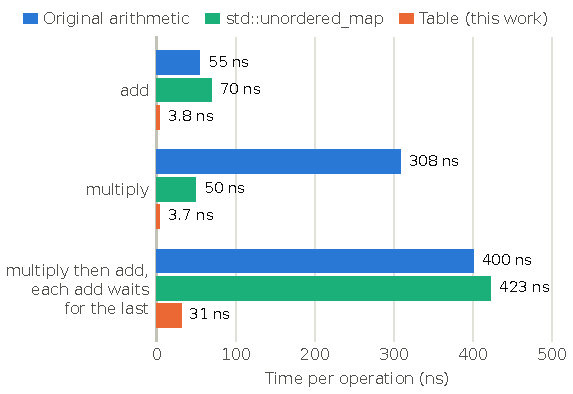
\includegraphics[width=\columnwidth]{figures/lookup_cost.pdf}
  \caption{Cost of one field operation with the original arithmetic, with a filled
  \code{std::unordered\_map} and with the filled tables.}
  \label{fig:lookup}
\end{figure}

For independent operations the hash map brings a multiplication from
\LookupOriginalMultiply~ns to \LookupMapMultiply~ns, and the table brings it to
\LookupTableMultiply~ns. The third group in the figure is the inner loop of a matrix
product, $s \leftarrow s + a_k b_k$, where each addition needs the previous sum before it can
start. \LookupChainedMapSentence. The table needs \LookupTableChained~ns, which is
\LookupChainedTableGain~times faster than the original.

The reason is memory. A hash map with 1.77 million entries keeps every entry in its own
heap node, and one lookup reads a bucket and then at least one node, each read waiting for
the one before~\cite{drepper2007memory}. A table lookup is one read from an array of
3.5~MB. Since every element is an integer below 1331, the pair of operands is already a
perfect array index and there is nothing to hash.
